%
% File acl2019.tex
%
%% Based on the style files for ACL 2018, NAACL 2018/19, which were
%% Based on the style files for ACL-2015, with some improvements
%%  taken from the NAACL-2016 style
%% Based on the style files for ACL-2014, which were, in turn,
%% based on ACL-2013, ACL-2012, ACL-2011, ACL-2010, ACL-IJCNLP-2009,
%% EACL-2009, IJCNLP-2008...
%% Based on the style files for EACL 2006 by 
%%e.agirre@ehu.es or Sergi.Balari@uab.es
%% and that of ACL 08 by Joakim Nivre and Noah Smith

\documentclass[11pt,a4paper]{article}
\usepackage[hyperref]{acl2019}
\usepackage{times}
\usepackage{latexsym}

 \usepackage{graphicx}
 \graphicspath{ {./images/} }

\usepackage{url}

\aclfinalcopy 
%\def\aclpaperid{***} %  Enter the acl Paper ID here

%\setlength\titlebox{5cm}
% You can expand the titlebox if you need extra space
% to show all the authors. Please do not make the titlebox
% smaller than 5cm (the original size); we will check this
% in the camera-ready version and ask you to change it back.

\newcommand\BibTeX{B\textsc{ib}\TeX}

\title{OP Hebrew Spam Detection Project 2019}

\author{Guy Twito \\
  The Open University / Israel \\
  \texttt{guyy18@gmail} \\\And
  Yuval Zaidel \\
  The Open University / Israel \\
  \texttt{yuvalzaidel10@gmail.com} \\}

\date{}

\begin{document}
\maketitle
\begin{abstract}
This project is about finding the best way to filter spam (unwanted) email messages and spam (unwanted) SMS (text messages) in Hebrew while using known methods for filtering spam email messages in English and comparing our results to known results from other experiences.
Likewise, we implemented additional methods that are appropriate specifically to Hebrew as a morphologic language and we found an improvement with the results.
Our datasets are email messages and SMS in Hebrew that were imported from personal sources of us and of our family and friends.

\end{abstract}



\section{Introduction}

The term "Spam mail" refers also to "Junk mail" or to "unsolicited commercial mail". Nowadays, there is a problem with receiving unwanted emails. The problem is very common because of the extensive use of email world wide. The great popularity of the electronic communications channel is utilized by email accounts that indiscriminately send emails with unwanted advertisements, which is unexpansive to send. 
Individuals can spend a lot of time filtering all the unwanted emails in their email box, while it's easy to get flooded with spam and miss legitimate messages. \\
The spam problem is reflected also in the field of SMS messages. We are receiving SMS messages to our private phones on a daily basis. Some of the SMS are spam messages that are used to advertising or to collect private information about us. Among those messages, we can find different kinds of sales, advertising for parties or explorations about the elections that occur once in a while. Individuals didn't ask for all these massages, which tags it as spam messages. A significant amount of the spam SMS messages is sent from different phone numbers which make it impossible to trace down the sender and just "block" him personally. \\
An issue about spam filtering is that if the automate filter represents a spam message as a legitimate massage it will be tolerable in terms of the user, but the opposite of represents a legitimate message as spam will be less tolerable in terms of most people. Hens, while building a model for spam filtering it is important to consider misclassification costs in order to evaluate the classification correctly.\\
 There is a lot of researches that used different classifiers and managed to tag massages as spam, with a high accuracy percentage, in different languages (English, Chinese). \\
In this project, we are focused on identifying spam massages in the Hebrew language. We couldn't find any previous experiments for that task online, that does not have a satisfying solution these days.\\
We'll check which of the methods that work for classifying spam in English, will work also when it comes to Hebrew. We'll also reveal some more methods that are adjusted specifically to the Hebrew language. We'll see the differences among the results of using the different methods, both in email and SMS messages, and we'll determine which method works the best when it comes to classifying spam emails and spam SMS messages in Hebrew.\\\\
All the code of the project is in \citep{git}

\section{Related Work}
\subsection{Data Gathering}
\label{ssec:Data Gathering}
We couldn't find any public Hebrew spam dataset, therefore we created two datasets, one that contains Hebrew email messages and one that contains Hebrew SMS messages.\\
At first, we opened two different WhatsApp Groups, one for sending all the spam SMS we could get our hands-on, and one for regular messages (non-spam SMS). We asked our friends and family to send us all the spam they can get. When we had enough data we exported the group's chat to email, and finally got standard files of exported WhatsApp chats.
In this way, we collected a variety of spam messages sent by SMS between July 16 and August 19. \\
In order to collect emails, we marked the spam messages in our mailbox with a specific label and the non-spam messages in another label. Afterward, we used \citep{lnk} for exporting emails to a "mbox" file. 
In this way, we collected emails that were sent to us between February 17 and July 19.\\
The data we collected had to be cleaned in a way that the models can read it easily, therefore we wrote a script that deletes the metadata of the message (sender and time details), deletes WhatsApp's system messages like "You created this group", "The message was deleted.", "Messages in this group are now secured with end-to-end encryption" and more. Afterward, the script removes duplicate messages, it makes each message to be one row by replacing '\n' chars with a constant and it shuffles them so that there won't be a sequence of conversation.\\
In order to publish the data we needed to censor the messages, so we replaced links, phone numbers, email addresses, and Emoji (for convenience) with a constant. Also, the names of people were replaced with random names in Hebrew that were taken from \citep{lnk2}

\subsection{YAP}
\label{ssec:YAP}
YAP is a tool that allows morphological decomposition of sentences in Hebrew. In addition, the tool specifies the PoS tag for each morpheme in the sentence and the sentence's dependency tree and more. We used this tool to morphologically decompose the sentences in the data we collected, so we could check if the decomposition gives an advantage when it comes to identifying spam messages.\\
Computational models for the automatic analysis of natural language texts which were originally developed for parsing Europen languages are not well suited for the analysis of languages that exhibit strong interaction between morphology and syntax -- also called Morphologically Rich Language (MRL). These languages, including Hebrew, Arabic, and other Semitic languages pose a specific challenge to the standard language processing pipeline. 
YAP can successfully cope with parsing MRLs.\\
For this task, we set up an instance in GCP and installed everything that YAP needs to operate, we have written an installation script and additional scripts to run it properly. In order to get the required output, the script takes all the datasets of emails and text messages, separates the common punctuation marks (? . ! ,) that are not part of a word (for example ' " ' is a symbol to acronyms, therefore it's a part of a word).\\
The script handles signs that have special meaning in bash \& \mid ${( ) " < > ' ` * }$ 

\noindent The script separates the sentences in each message, run YAP on each one, extracts the relevant information to us and save it in a suitable file.

\section{Method and Model}
The spam filtering task, according to many articles, is done by classification into two categories – spam messages and legitimate messages. In order to run a classifier, we need to take different actions that take time – we need to read the data, divide it for training and testing, create a features vector and use different evaluation methods.\\
In order to test all our experiments, we had to test several classifiers on a number of different data sets. We implemented the code in a way that all the operations that are needed for a model to run are performed once for all models in each run with the wanted parameters, for all the required data sets. With that implementation we saved run-time and we were able to compare between the models better because the splitting of the data to train and test occurred only once for all.\\
Also, if necessary, one particular classifier can be executed easily instead of all of the classifiers at once.\\
According to the parameters, we read the data of emails and SMS from the suitable files and processed the information requested for the current run – considering if morphological decomposition is needed or not, building the dependency trees, make integration of the data sets or not, and limit the size of the data.\\
For each data set, we were able to divide the data by a certain percentage, or make k-cross-validation which is a method of dividing the data into k parts and then performing k iterations of the model, so that in each time we train the model for k-1 parts of the data, and testing it with the remaining part. This method allows one to see how the model deals with different data distributions rather than relying on incidental results. . We performed our experiments for k = 5, because according to \citep{lnk3} the uses of k = 10 or k = 5 were found to provide a good evaluation.
\begin{quote}
Typically [...] one performs k-fold cross-validation using k = 5 or k = 10, as these values have been shown empirically to yield test error rate estimates that suffer neither from excessively high bias nor from very high variance.
\end{quote}\\
For each iteration, after dividing the data, making one feature vector was enough for fitting all the models required by the parameters of the run. After the training, we performed a test for each of models and printed different evaluations. Finally we have presented a summary of the evaluations - the average and the lowest value of each metric. We also displayed the incorrectly classified messages and how many times they were tagged wrongly by every model, in order to check problematic messages and which other features can be added.\\
We chose the features according to articles we read, according to our intuition of what a spam message looks like and by looking at the data itself. The tested models were selected according to \citep{andrew2007scalable} and \citep{Ando2005} in order to compare our results in the Hebrew language with the results of the English language in the articles.\\\\
We selected much features, in the suggest of \citep{andrew2007scalable}:
\begin{quote}
Aggressive feature pruning should be avoided when building filters to be used in scenarios where legitimate mails are assigned a much higher weight than spams (such as $\lambda$ = 999), so as to maintain a better-than-baseline result (TCR999${>}$1). The possible reason may be that the higher $\lambda$ is, the more features should be used to let the classifier produce a reliable prediction.
\end{quote}\\
\textbf{Selected features:} 3-grams for words; 3-grams for letters; Bag of words-count of the amount of common spam and non-spam words. The words are set to be without characters, longer than one character (or two), over 5 instances in all messages of a certain type, and not in the common words of the other group; the ratio between statistics of all spam and non-spam messages and the count in the sentence itself (amount of emojis and type, amount of lines, amount of links and length); Tokens counting; Counting letters, no links, telephone numbers and emails (because their size does not indicate the length of the message content); Amount of links; Average length of links; Average position of the links relative to the message; Number of types of telephone numbers; The longest word, without counting the fixed variables we set; Number of non-letter signs (without the fixed variables, also without links, phones and emails); Percentage of marks in the message; punctuation marks counting , . : ! ? ' " - ; Count the amount of emojis; Percentage of emoji in the message; The ratio between Hebrew and English letters; Amount of sentences; Amount of numbers (without links, phone numbers or emails); Percentage of numbers in the message; \textbf{In addition, features tested by POS parameter:} Count of the number of instances of each pos tag that appears in each data set; 3-grams on tag POS; \textbf{Also, features tested by the dependency trees parameter} parameter (for each sentence in a message there is a tree): The highest tree height of all the trees; The largest number of children among all the trees; The number of different relation tag; 3-grams for dependency trees; 

\textbf{Models:}\\
\begin{itemize}
\item \textbf{Multinomial Naïve Bayes} - a specialized version of Naive Bayes that is designed more for text documents. Whereas simple naive Bayes would model a within as the presence and absence of particular words, Multinomial Naive Bayes explicitly models the word counts and adjusts the underlying calculations to deal within.
\item \textbf{Logistic Regression} - Logistic Regression is a Machine Learning algorithm which is used for the classification problems, it is a predictive analysis algorithm and based on the concept of probability. The hypothesis of logistic regression tends it to limit the cost function between 0 and 1.
\item \textbf{K-nearest neighbors} - a non-parametric method used (in our case) for classification. A small value of k means that noise will have a higher influence on the result and a large value make it computationally expensive. To choose K wisely, we used various internet websites (for example \citep{lnk3}) and we found that a squared root of the amount of the data is a fine choice. We didn't have any memory errors so we tripled it.
\item \textbf{SVM} - The objective of the support vector machine algorithm is to find a hyperplane in N-dimensional space (N — the number of features) that distinctly classifies the data points. SVM chooses the decision boundary that maximizes the distance from the nearest data points of all the classes. An SVM doesn't merely find a decision boundary, it finds the most optimal decision boundary.
\item \textbf{Adaptive Boosting} - AdaBoost can be used in conjunction with many other types of learning algorithms to improve performance. The output of the other learning algorithms ('weak learners') is combined into a weighted sum that represents the final output of the boosted classifier. In our case, we chose the "n\_estimators" (amount of weak learners) to be 50 (and not larger because of memory errors).
\end{itemize}

\noindent \textbf{Evaluations:}\\
First, we checked the \textbf{Baseline} – which measures the percentage of accuracy if we classify everything as non-spam. If we get a result that is under this percentage, it means that we shouldn't do the Spam Filtering at all. We checked also the \textbf{positive margin} that indicates how much we have exceeded the baseline.\\
We introduced also the \textbf{confusion matrix} – a matrix that shows how much spam was classified as non-spam and spam, and how much non-spam was classified as non-spam and spam (FP TP TN FN). In this way, we can see the results clearly and calculate the following metrics:
\begin{itemize}
\item \textbf{Recall} - a fraction of real spam massages that has been retrieved over the total amount of the real spam messages in our data.
\item \textbf{Precision} - a fraction of real spam massages among the retrieved spam messages, which are not necessarily real spam messages.
\item \textbf{F1 score} - It considers both the precision and the recall of the test to compute the score.
\item \textbf{WAcc} - Weighted Accuracy measure specially tailored for the scenario that non-spam messages classified as a spam message (it assigns false positive a higher cost than false negative).\\
\boxed{\mathit{$WAcc$}_{\lambda$} = $\frac{\lambda \cdotp \mathit{n}_{L \rightarrow L}+\mathit{n}_{S \rightarrow S}}{\lambda \cdotp \mathit{N}_{L} + \mathit{N}_{S}}$ }\\
While N$_{L}$ is the total number of legitimate messages and N$_{S}$ denotes the total number of spams. WAcc treats each legitimate message as if it were ${\lambda}$ messages: when false positive occurs, it is counted as ${\lambda}$ errors; and when it is classified correctly, this counts as ${\lambda}$ successes. The higher ${\lambda}$ is, the more cost is penalized on false positives.

\item \textbf{TCR} - a single measurement of the spam filtering effects:\\
\boxed{$TCR$ = $\frac{WErr^b}{WErr}$ = $\frac{\mathit{N}_{S}}{\lambda \cdotp \mathit{n}_{L \rightarrow S}+\mathit{n}_{S \rightarrow L}}$ 
}\\
While WErr$_{b}$ (= $\frac{N_S}{\lambda \cdotp N_L + N_S}$) is the baseline versions of weighted error rate. We use Total Cost Ratio to avoid the problem that when λ is assigned a high value, WAcc can be so high that it tend to be easily misinterpreted (it is better to compare the weighted accuracy and error rate to a simplistic baseline).

\end{itemize}


\section{Data}
\subsection{Clean Data}
\label{ssec:Clean Data}
 emails and SMS messages are marked as Spam or Non-Spam, the structure of the data is that every massage is in a different line and there are constants in the form "xxxxENDVAR":
\begin{itemize}
\item ENTERNEWLINEENDVAR - separates between sentences.
\item MAILSUBJECTENDVAR - used in email messages, comes between the head and the body of the massage. The choice to join the subject with the body is that \citep{andrew2007scalable} that found that it achieves the best results.
\item EMAILENDVAR - email address.
\item LINK25ENDVAR - link. The number in the middle expresses the length of the link.
\item PHONENUMBER4ENDVAR - phone number. The number is the middle expresses the type of the phone numbers structure as we defined it 
(...-03 = \textbf{1}, 1800-… = \textbf{2}, 052-… = \textbf{3}, +972… = \textbf{4}).
\item EMOJI\_ENDVAR - represents an Emoji, the sign in the middle is the Emoji itself.
\end{itemize}

\subsection{Morphological decomposition}
\label{ssec:Morphological decomposition}
Morphological decomposition of the Clean Data, each morpheme build as a\~b\~c\~d, while:
\begin{itemize}
\item a - the morpheme itself.
\item b - PoS tag.
\item c - head (information needed to build a dependency tree).
\item d - relation (one of dependency trees tags).
\end{itemize}
\noident We executed the model with the different features for  every type of our data (SMS, emails, morphological decomposition of SMS, morphological decomposition of emails).

\section{Experiments}
For running the experiments we started an instance in GCP that runs Ubuntu, 16.04 LTS,  עם4 vCPUs, 30 GB memory. The experiments we conducted are running the different models on each of the datasets with different parameters.\\
The parameters tested are:
\begin{itemize}
\item Whether to include a combination of the email dataset and the SMS dataset.
\item Limitation on the amount of non-spam messages, In order to adjust to the amount of memory on the machine and also to change the ratio between spam to non-spam messages.
\item Whether to use morphological decomposition
\item Whether to use features of POS.
\item Whether to use features of dependency trees.
\item Define K for k-cross-validation.
\item Which models to use - Use all models or a specific model.
\end{itemize}
\noindent In general, we used 5-fold cross-validation and ran most of the experiments for all the models (the consideration of not running all parameters is a consideration of time and memory).\\
All the results files are numbered in \citep{git}.\\



\subsection{Experiment 1: Basic comparison}
\label{ssec:Experiment 1}
Results file is \textbf{1}, Compared to \citep{andrew2007scalable} and \citep{Ando2005}, Parameters are regular (not morphologically decomposed) emails and SMS dataset, non-spam is limited to 6000, run all models.\\
Table 1 shows the datasets spam ratio.\\
Table 2 and Figure 1 show the SMS results.\\
Table 3 and Figure 2 show the Email results.\\
We can see from the results that the "low" results of F1 and WAcc in all models (besides KNN) do not go lower than 96\% and 98\%.
If we'll look at the TCR results, we can see that when $\lambda$ equals 1 all models got a higher score from 1, which means that if we won't give higher price for classifying a legitimate message as spam, the model could be used in an application in the real world.
Since there is a higher price for this situation we will look at the situation when $\lambda$ = 99 and also when $\lambda$ = 999. In these situations, there is no model that received a score higher than 1 in SMS, but we can still see that the "average" and "low" values of MultinomialNB are higher than the other models. the values of LogisticRegression, SVM, AdaBoost are basically the same, and the value of KNN is the lowest.\\
The Email results of each model are similar except that we can see that the TCR values are higher than SMS, and also, MultinomialNB received 3 times TCR99${>}$ 1 and once TCR999${>}$ 1.\\
The result may seem accidental because not all iterations came out with the same results, although no other model has received such a score and they are all working on the same division of data.\\
\textbf{Comparison to the articles:}\\
F1 values appear to be in the 96\% -98\% range with the SMS baseline being 84.3\% and the EMAIL baseline 52.4\%, so the classifiers seem to work well in most cases. If we compare our results to the articles, they appear to reach a minimum of 95\% -97\% when the baseline of their datasets were 56.3\% and 68.7 \%.\\
In \citep{Ando2005}, they checked the WAcc999 value for several types of AdaBoost and this value did not drop from its average of 99.47 \%, reaching to 99.98\%.
In our experiment, AdaBoost reached an average of 98.9\% for SMS and 96.5\% for Email. The highest result was the result of MultinomialNB which reached an average of 99.5\% for SMS and did not decrease from 99.16\%. For Email, the model reached an average of 99.16\% and did not drop from 98.59\%.\\
In \citep{andrew2007scalable}, they checked the TCR999 value for all the models we tested and their value was higher than 1for the models, AdaBoost, SVM, and LogisticRegression compared to our results which were low for these models. In this article, the TCR999 values of MultinomialNB have reached 0.02, compared to our experiment that had higher results for the model (although not good enough) and several times above 1.\\
To sum up the experiment, the MultinomialNB model seems to be stronger than all the tested models, but its results are still not considered good in the case of cost-sensitive evaluation, and even when it comes to good results, the results are unstable (sensitive to noise).
This, in contrast to the results of the articles, raises the possibility that the MultinomialNB Spam filter in the Hebrew language is better than the SVM, AdaBoost, LogisticRegression models chosen as the ideal models for English.\\
\textbf{NOTE:} After showing once the F1 and WAcc scores in this experiment we won't show it because it doesn't change much, but it can be reached in the results files.

\subsection{Experiment 2: Higher Spam Ratio}
\label{ssec:Experiment 2}
Results file is \textbf{2}, Compared to Experiment 1, Parameters are regular SMS dataset, non-spam is limited to 3000, run all models.\\
Table 4 shows the dataset spam ratio.\\
Table 5 shows the SMS results.\\
In this experiment, we want to check if the spam rate affects the accuracy of the model. If we'll compare our output results between both of the experiments, we can see an improvement in almost all the metrics when there are fewer legitimate messages and a higher spam percentage.\\
To sum up the experiment, the fewer legitimate messages, the better the results. It turned out that for less data (with higher spam rate) the results improved slightly, so we conclude that testing the models with a large corpus that includes many types of legitimate messages and spam messages will require a much stronger prediction.

\subsection{Experiment 3: Lower Spam Ratio}
\label{ssec:Experiment 3}
Results file is \textbf{3}, Compared to Experiment 1 and 2, Parameters are morphologically decomposed SMS and Email datasets, non-spam is limited to 10000, run only for MultinominalNB model.\\
Table 6 shows the dataset spam ratio.\\
Table 7 shows the SMS results for different corpus sizes.\\
We performed this experiment only for one model due to memory errors, and we chose MultinominalNB, which so far seems to be the strongest model among the tested models.
We'll take a look at the results of MultinomialNB on SMS side by side in Table 7.
We can see that the change in the size of the corpus and the spam rate affects in a way that the larger the corpus - F1 percentage decreases on "average" but more accurate in its "low" value. In terms of TCR values with $\lambda$ = 99 and 999, the larger corpus is more accurate at the "average" value but less accurate at the "lowest" value.\\
We can conclude that a too-small corpus can lead to the conclusion that the model is better than it really is, though its realization in a real app will not be good enough. 
In addition, the larger the data, the less stable the model (= mistaken for more legitimate messages).

\subsection{Experiment 4: Morphologically decomposed data without features}
\label{ssec:Experiment 4}
Results file is \textbf{4 (email) , 5 (SMS)}, Compared to Experiment 1, Parameters are morphologically decomposed SMS and Email datasets, non-spam is limited to 6000, no PoS or dependency tree features, run for all models.\\
Table 8 shows the SMS results.\\
Table 9 shows the Email results.\\
For SMS, there is a slight improvement in all model indices, except for the MultinomialNB model where the "average" results actually dropped but the "low" results were improved, and except from the LogisticRegression model where the "average" results actually improved but the "low" results dropped.\\
For a similar comparison for Email, there seems to be a decrease in the accuracy percentages for almost all the metrics in all models, for both F1 and TCR results. This is the opposite of the results for SMS.\\
To conclude, in general, we can say that morphological decomposition without additional features can slightly contribute to the stability of the model, without improvement in prediction in case of a dataset from a certain type (SMS), and in the case of another dataset (Emails) it is actually harmful.

\subsection{Experiment 5: Morphologically decomposed data with features}
\label{ssec:Experiment 5}
Results file is \textbf{6 (pos) , 7 (dependency trees) , 8 (both)}, Compared to Experiment 1 and 4, Parameters are morphologically decomposed SMS and Email datasets, non-spam is limited to 6000, PoS and dependency tree features are mentioned by the results file number, run for all models.\\
Table 10,11 shows the SMS and Email results for results file 6.\\
Table 12 shows the Email results for results file 7.\\
Table 13 shows the Email results for results file 8.\\
Looking at Table 10, for morphologically decomposed SMS with POS features, compared to Experimetn 1, we can see that there is a very small increase in most TCR "low" values, but most TCR averages have dropped.
Looking at Table 11, for morphologically decomposed Email we can see a decrease for all models in almost all indices except MultinomialNB, all of which have actually improved significantly - TCR99${>}$1 in all 5 iterations tested, and TCR999${>}$1 came out once.
In either case the results in both data sets were better than the results of Experiment 1.\\\\
For morphologically decomposed SMS with dependency trees features, we could not see any significant improvement over previous experimental results.
In contrast, looking at Table 12, for morphologically decomposed Emails with dependency trees features, we obtained 4 times TCR99> 1 and 2 times TCR999> 1 MultinomialNB model. This result is reminiscent of the result of the experiment with POS features.\\\\
Since the results for morphological decomposition with POS features and dependency trees features showed improvements for emails, we'll check what happens when both are turned on.\\
For SMS no improvement can be seen.
Looking at Table 13, the results for the MultinomialNB model were TCR99${>}$1 three times (compared to 4 or 5 times when the features are separate), and TCR999${>}$1 two times.\\
We can easily see that when putting together POS and dependency trees features the results are worse than each one individually, so together they have no advantage.\\\\
To conclude the experiment, morphological decomposition with POS features can be useful because it makes the model more stable for the Emails dataset since it improves F1 values and "low" TCR metrics (though it lowers the average of those values). Features of dependency trees can also increase the accuracy of the model, although its stability is uncertain. 
For the SMS dataset we could not improve using the morphological decomposition, therefore we cannot conclude from this whether the features we have chosen do not fit this type of data or it cannot contribute to this type of data due to noise or similarity between the POS or dependency trees of the legitimate and spam messages.

\subsection{Experiment 6: Morphologically decomposed union dataset}
\label{ssec:Experiment 6}
Results file is \textbf{9}, Compared to Experiment 4, Parameters are union of morphologically decomposed SMS and Email datasets, non-spam is limited to 3000 (6000 together), no PoS or dependency tree features, run only for MultinomialNB model.\\
Table 14 shows the morphologically decomposed union results.\\
We can see that there is no change in the accuracy percentages of F1 and WAcc but there is an improvement in the TCR since TCR99${>}$1 was 3 times, compared to the SMS which was 0 times, and the emails for which TCR99${>}$1 was twice and TCR999${>}$1 once.
In the morphological decomposition SMS, there were 517 different classification mistakes for all the iterations out of 7108 messages (7.2\%). Iin the morphological decomposition emails, there were 383 different classification mistakes for all the iterations out of 1465 messages (26.1\%). While combined there were only 185 different classification mistakes in all iterations out of 5578 messages (3.3\%) which were divided into 42 emails and 143 SMS.
We can see a significant decrease in the number of errors, although the messages count in the dataset is similar.\\
To conclude the experiment, we can say that a combination of morphologically decomposed datasets gives better results than each one separately when no features are being tested, so we conclude that a combination of different sources of information can lead to a more general learning of the model and thus produce better results. It might put an emphasis on the content of the message and less on the structure of the platform on which it was sent.

\subsection{Experiment 7: Trying to Improve AdaBoost}
\label{ssec:Experiment 7}
Results file is \textbf{10}, Compared to Experiment 4, Parameters are morphologically decomposed SMS and Email datasets, non-spam is limited to 6000, no PoS or dependency tree features, run for AdaBoost model.\\
Table 15,16 shows the SMS and Email results.\\
We wanted to check whether we can get better results with the AdaBoost model if we will test it with best parameters we found, but instead of 50 estimators we will try it with 200 estimators, and maybe compare to the results of the articles which were very good for the model
Looking at tables 15 and 16 and comparing with the noted experiment, we got better results than 50 estimators but still not close to the results of the AdaBoost model in the articles. Therefore, we conclude that the model is less suitable for spam filtering in Hebrew, or that there is a way to use the model better than we did and make it improve more.

\section{Discussion}
When trying to filter spam in Hebrew, for all models tested, the accuracy percentages remain high as in English (96\%-98\%). The difference between the languages is reflected in the lack of accuracy of the models in the remaining percentages. When a legitimate message is classified as spam, the metrics show a different picture. From now on we will refer to the results only for cost-sensitive evaluation.\\
We found that the MultinomialNB model classifies spam in Hebrew better than the other tested models, although articles that concentrated in the English language categorized the MultinomialNB model as not good enough for the task. The same articles achieved with the AdaBoost, SVM and LogisticRegression models good results, whereas the results for Hebrew were less good for those models.
Possible hypotheses why this might happen:
\begin{itemize}
\item In Hebrew, it's really better to filter by using the MultinomialNB model than the other models.
\item As part of the conclusions of \citep{andrew2007scalable} for each dataset, there may be a different model whose results will be far better than other models.
\item The number of features we used was greater than the number that the articles were using, which could reinforce MultinomialNB whose premise is that there is no effect between the features.
\end{itemize}

\noindent We found that in order to improve spam filtering in Hebrew both in terms of accuracy and stability (noise resistance for input), we can use the morphological decomposition of the data. Morphological decomposition without additional features can bring us to more stable results for SMS but makes email prediction worse. We speculate that this is probably due to the noise it makes for the long emails, whereas the short SMS messages get to contain more relevant information.\\
We found that combining different datasets can give better results than each one individually. We hypothesize that this is happening because it results in more general learning of the model that puts more emphasis on content than platform structure.\\
We found that the more legitimate messages, the better the results because there are fewer possibilities for an expensive mistake to happen, so in the real-world, where legitimate messages rate can be high and the spam rate drops, It will be more difficult to achieve good and stable prediction.\\
We do not rule out the possibility that we have used the models that the articles have recommended differently, so it might make them less good in our experiments. We used the default parameters for the models, but modifying the parameters of the models can cause a difference in the results, as we saw in the last experiment where there was an improvement (though not significant) in the AdaBoost model when we increased the number of estimators.\\
Most often, the results for the Email dataset were better than the results for the SMS dataset. Our hypotheses for the reasons for it are that the structure of legitimate SMS messages and spam messages can be similar, compared to a spam email structure whose features can be more prominent than legitimate emails.
We can also say that the Email dataset is relatively small and may not be sufficiently inclusive which may make it easier to predict. The emails came from two people's inboxes, so it probably doesn't represent the messages of an entire population. The sms are more inclusive and include writing styles of people from different age groups (at the same time, there can be many more writing styles that do not come to an exspration) and that may make the difference.\\
In general, we could say that we expected stronger SMS prediction in the project and surprised us to see that it is actually more difficult than email prediction. In addition, we expected the POS features and the dependency trees features to be much stronger, and we wonder if some other features for this data could be a better metric than our features were.\\
At last, when going over the messages which there were classification mistakes, we found a number of reasons for repeated mistakes:
\begin{itemize}
\item Spam messages that have been sent as legitimate messages. For example, a message about a party whose classification is spam and actually comes from an unwanted sender, but a person who was interested in the party passed it legitimately to his friend, an action that makes this message to a non-spam message. Such a situation can only be identified by metadata that we do not have as part of the model information, such as who the sender is, whether there is a correspondence with him, how many legitimate messages the person got from him, etc. In emails as part of mbox export, we receive additional metadata that we did not process, but according to \citep{andrew2007scalable}, which in some parts did process the metadata, they found, for example, information about the e-mail server and improved their accuracy.
\item Writing style of some companies - desirable messages that sent by senders who also send spam messages (advertisements) can be in the same format with a little change and be mistakenly classified as spam, for example, "Pelephone" send out advertisements (spam) and also notifications for ending a browsing package that will incur additional charges (not spam).
\item Different writing styles of people - messages from people who usually write in a structure that is less acceptable within the dataset of the legitimate messages may be considered as spam (For example, "Hey, reminding you we meet on Friday .... waiting to see you!").
\item Notices that one wants to receive for a service or a product that he purchased, or information about something he is requesting - these messages are general to many users and formulated in a spam message structure but it is desirable for users (For example, "Hey, glad you chose to order ...... Your benefit code is ....", "The last reminder! Please hurry to return the costumes. On March 28, the unpaid deposits will be deposited ... ").
\item Spam messages that do not have a certain structure or words may be misclassified, for example:\\
"Blue-white or Likud? Independent, choose economic power"\\
"Who was thrown from the Knesset committees but not from the books of history?"\\
"Light Chanukah Candles: ENTERNEWLINEENDVAR Tonight 2 Candles and so on"
\item Sophisticated spam messages that present themselves or address a person by name and thus address in a more personal way as addressed by legitimate messages, For example:\\
"Hey what's going on? ENTERNEWLINEENDVAR My name is Daniel and I ...."\\
"Hey, it's Hila from promotion ...."\\
"Hello Hoshaya Amir Tohar, tomorrow the election campaign will be held ...."
\end{itemize}


\section{Conclusion}
The presented experiments show a comprehensive evaluation for five different classifiers measured with a cost-sensitive evaluation for 2 different types of Hebrew datasets. Different features and  methods were tried, some are commonly used in researches all over the web and some are particularly suited to the Hebrew language. We found that:
\begin{itemize}
\item In the Hebrew spam filtering task, we will get the best results for the MultinomialNB model.
\item In a data set of SMS, we found that if we decompose it morphologically we would get results with more robust metrics, which would be even better if the model training included POS features
\item When morphologically decompose the SMS dataset, we can get results with more robust metrics, which are be even better if we include POS features.
\item When morphologically decompose the Email dataset we can harm the predictability, but if we include POS features or dependency trees features (but not both kinds of features together) we can get results with a much higher percentage of accuracy than without the features or without the morphological decomposition.
\item If we combine the morphologically decomposed we can get better results even without the POS or dependency trees features.
\item As the number of legitimate messages increase (i.e. spam rate decreases), the prediction becomes less stable because there is more room for expensive mistakes.
\end{itemize}

\section{Suggestions for Future Work}
\begin{itemize}
\item When trying to run different models we came across memory errors. Therefore, in the future, it will be worth to try and run some more models and check whether some model gets better results.
\item Creating a UI which its input is a regular sentence (email or SMS message), the program will clean the sentence so it will be similar to the data we collected, then we'll use YAP on this sentence, after that we'll run the trained model on it and eventually the output will be if the sentence is spam or not (as an inspiration from YAP). 
\item Working with a bigger corpus and trying to get a good performance may be interesting for the use of a real application.
\end{itemize}

\bibliography{acl2019}
\bibliographystyle{acl_natbib}

\begin{table*}[t!]
\centering
\begin{tabular}{lll}
  dataset & Vocabulary Size & Spam Rate\\
  \hline
  SMS & 7110 &15.7 \% \\
  Email & 1469 &48.6 \% \\
\end{tabular}
\caption{Experiment 1 Datasets information}
\end{table*}


\begin{table*}[t!]
\centering
\begin{tabular}{lllllll}
 *& Ave TCR1 &Low TCR1&Ave TCR99&Low TCR99&Ave TCR999&Low TCR999\\
  \hline
  KN-Neighbors& 3.1471&	2.3626&	0.084&	0.0536&	0.0085&	0.0054	\\
LogisticRegression& 10.6931&	8.8&	0.1929&	0.1472&	0.0193&	0.0147	\\
SVM& 12.7451&	9.9545&	0.239&	0.1571&	0.0239&	0.0156	\\
MultinomialNB& 6.9622&	5.2791&	0.4523&	0.2219&	0.0473&	0.0226	\\
AdaBoost& 9.7135&	8.4444	&0.1895&	0.1302&	0.019&	0.0129	\\

 \\
\end{tabular}
\caption{Experiment 1 SMS results}
\end{table*}

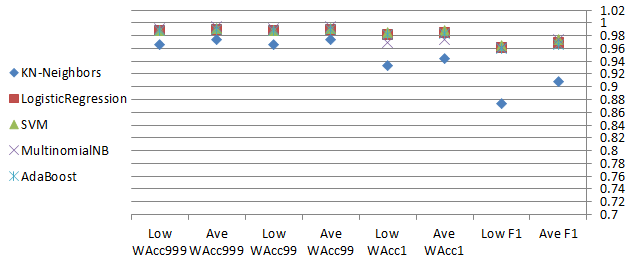
\includegraphics[scale=0.4]{1}
Figure 1: Experiment 1 SMS results

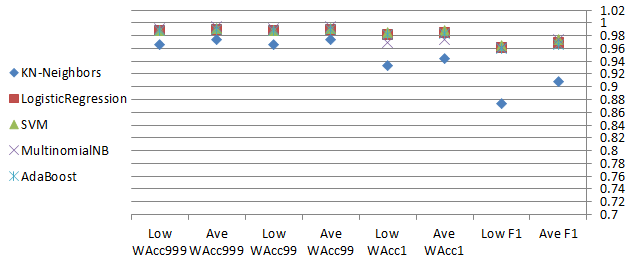
\includegraphics[scale=0.4]{1}
Figure 2: Experiment 1 Email results

\begin{table*}[t!]
\centering
\begin{tabular}{lllllll}
 *& Ave TCR1 &Low TCR1&Ave TCR99&Low TCR99&Ave TCR999&Low TCR999\\
  \hline
  KN-Neighbors& 2.653&	2.2308&	0.1874&	0.0716&	0.0201&	0.0072	\\
LogisticRegression& 14.5744&	10.7692&	0.3537&	0.2003&	0.0355	&0.02	\\
SVM& 15.2936&	11.1538&	0.4074&	0.235&	0.041	&0.0235	\\
MultinomialNB &15.9178&	12.6667&	4.2049&	0.7255&	3.445&	0.0739	\\
AdaBoost& 11.8239&	9.125&	0.2919&	0.208&	0.0293&	0.0209	\\

 \\
\end{tabular}
\caption{Experiment 1 Email results}
\end{table*}


\begin{table*}[t!]
\centering
\begin{tabular}{lll}
  dataset & Vocabulary Size & Spam Rate\\
  \hline
  SMS & 4114 &27.1 \% \\
\end{tabular}
\caption{Experiment 2 Dataset information}
\end{table*}


\begin{table*}[t!]
\centering
\begin{tabular}{lllllll}
 *& Ave TCR1 &Low TCR1&Ave TCR99&Low TCR99&Ave TCR999&Low TCR999\\
  \hline
  KN-Neighbors& 3.4473&	2.7444&	0.107&	0.0648&	0.0108&	0.0065	\\
LogisticRegression& 12.92&	9&	0.2225&	0.1278&	0.0222&	0.0127	\\
SVM& 14.7452&	9.4762&	0.2516&	0.1537&	0.0251&	0.0153	\\
MultinomialNB &8.2067&	5.2&	0.781&	0.3118&	0.0879&	0.0324	\\
AdaBoost& 11.3938&	8.25&	0.2019&	0.1325&	0.0202&	0.0132	\\

 \\
\end{tabular}
\caption{Experiment 2 SMS results}
\end{table*}

\begin{table*}[t!]
\centering
\begin{tabular}{lll}
  dataset & Vocabulary Size & Spam Rate\\
  \hline
  SMS & 11096 &10 \% \\
\end{tabular}
\caption{Experiment 3 Dataset information}
\end{table*}

\begin{table*}[t!]
\centering
\begin{tabular}{lllllll}
 *& Ave TCR1 &Low TCR1&Ave TCR99&Low TCR99&Ave TCR999&Low TCR999\\
  \hline
MultinomialNB 3000& 8.2067&	5.2	&0.781&	0.3118&	0.0879&	0.0324	\\
MultinomialNB 6000&6.9622&	5.2791&	0.4523&	0.2219&	0.0473&	0.0226	\\
MultinomialNB 10000& 6.0191	&5.3556&	0.5949&	0.2079&	0.0675&	0.0211	\\

 \\
\end{tabular}
\caption{Experiment 3 , Comparison between different corpus sizes}
\end{table*}

\begin{table*}[t!]
\centering
\begin{tabular}{lllllll}
 *& Ave TCR1 &Low TCR1&Ave TCR99&Low TCR99&Ave TCR999&Low TCR999\\
  \hline
  KN-Neighbors& 2.9997	&2.8987&	0.0801	&0.0559&	0.0081&	0.0056	\\
LogisticRegression& 14.3682	&9.6957&	0.2337	&0.1248&	0.0233&	0.0124	\\
SVM& 14.9954&	12.0526	&0.3378	&0.1933&	0.0341&	0.0193	\\
MultinomialNB &7.0718&	5.9512&	0.3571&	0.2517&	0.0368&	0.0256	\\
AdaBoost& 9.9449&	8.7037&	0.1988&	0.1332&	0.0199&	0.0132	\\

 \\
\end{tabular}
\caption{Experiment 4 SMS results}
\end{table*}

\begin{table*}[t!]
\centering
\begin{tabular}{lllllll}
 *& Ave TCR1 &Low TCR1&Ave TCR99&Low TCR99&Ave TCR999&Low TCR999\\
  \hline
  KN-Neighbors& 2.6406&	2.3	&0.1334&	0.0693&	0.0139&	0.007	\\
LogisticRegression& 12.12&	9.6&	0.4289&	0.1725&	0.0448&	0.0171	\\
SVM& 12.4769&	9.8&	0.3274&	0.1997&	0.0331	&0.0199	\\
MultinomialNB &16.2667&	8.7059&	3.2705&	0.4759&	2.6692&	0.0492	\\
AdaBoost& 11.6465&	8.9375&	0.2826&	0.1592&	0.0286&	0.0159	\\

 \\
\end{tabular}
\caption{Experiment 4 Email results}
\end{table*}

\begin{table*}[t!]
\centering
\begin{tabular}{lllllll}
 *& Ave TCR1 &Low TCR1&Ave TCR99&Low TCR99&Ave TCR999&Low TCR999\\
  \hline
  KN-Neighbors& 3.0271&	2.7821	&0.074&	0.0619&	0.0074&	0.0062	\\
LogisticRegression&11.4912&	9.9048&	0.1825&	0.1493&	0.0182&	0.0149	\\
SVM& 13.6928&	11.6111	&0.2394&	0.175&	0.0239&	0.0174	\\
MultinomialNB &6.1371&	5.7073&	0.409&	0.2794&	0.0432&	0.0287	\\
AdaBoost& 11.6051&	8.2692&	0.2358&	0.1603&	0.0236&	0.0159	\\

 \\
\end{tabular}
\caption{Experiment 5 SMS results, without dependency trees or POS features}
\end{table*}

\begin{table*}[t!]
\centering
\begin{tabular}{lllllll}
 *& Ave TCR1 &Low TCR1&Ave TCR99&Low TCR99&Ave TCR999&Low TCR999\\
  \hline
  KN-Neighbors& 2.4969&	2.2593&	0.1037&	0.0701&	0.0106&	0.0071	\\
LogisticRegression&12.3884	&10.3571	&0.2991&	0.2023&	0.0301	&0.0202	\\
SVM& 13.4563&	10.3571	&0.4888&	0.2023&	0.0508&	0.0202	\\
MultinomialNB &16.5102&	13.2727	&4.5389&	1.3394&	3.5413&	0.1447	\\
AdaBoost& 11.7752&	8.1667&	0.4538&	0.1779&	0.0471&	0.0178	\\

 \\
\end{tabular}
\caption{Experiment 5 Email results, without dependency trees or POS features}
\end{table*}

\begin{table*}[t!]
\centering
\begin{tabular}{lllllll}
 *& Ave TCR1 &Low TCR1&Ave TCR99&Low TCR99&Ave TCR999&Low TCR999\\
  \hline
  KN-Neighbors& 2.6044&	2.2568&	0.1023&	0.0662&	0.0104&	0.0067	\\
LogisticRegression&14.999&	9.7333&	0.3486&	0.1794&	0.035&	0.0179	\\
SVM& 15.315	&10.6429&	0.3558&	0.1794&	0.0357&	0.0179	\\
MultinomialNB &19.2333&	14&	8.5035&	0.7317&	7.8734&	0.0748	\\
AdaBoost& 13.7323&	6.9524&	0.3033&	0.1459&	0.0305&	0.0146	\\

 \\
\end{tabular}
\caption{Experiment 5 Email results, with dependency trees features, no POS}
\end{table*}

\begin{table*}[t!]
\centering
\begin{tabular}{lllllll}
 *& Ave TCR1 &Low TCR1&Ave TCR99&Low TCR99&Ave TCR999&Low TCR999\\
  \hline
  KN-Neighbors& 2.5949	&2.12&	0.1282&	0.0527&	0.0133	&0.0053	\\
LogisticRegression&2.5949&	2.12&	0.1282&	0.0527&	0.0133&	0.0053	\\
SVM& 11.633	&8.9375	&0.3526&	0.1544&	0.0359&	0.0153	\\
MultinomialNB &16.107&	13.0909	&7.0257&	0.4918&	6.5584&	0.0499	\\
AdaBoost& 9.862&	7.7778&	0.3007&	0.1277&	0.0306&	0.0127	\\

 \\
\end{tabular}
\caption{Experiment 5 Email results, with POS features, no dependency trees}
\end{table*}

\begin{table*}[t!]
\centering
\begin{tabular}{lllllll}
 *& Ave TCR1 &Low TCR1&Ave TCR99&Low TCR99&Ave TCR999&Low TCR999\\
  \hline
MultinomialNB &11.0224&	9.2143&	1.1223	&0.5345&	0.1221&	0.0551	\\

 \\
\end{tabular}
\caption{Experiment 6 both datasets results}
\end{table*}

\begin{table*}[t!]
\centering
\begin{tabular}{lllllll}
 *& Ave TCR1 &Low TCR1&Ave TCR99&Low TCR99&Ave TCR999&Low TCR999\\
  \hline
AdaBoost 200 &11.1249&	9.2174&	0.2032&	0.1635&	0.0203&	0.0163	\\
AdaBoost 50 &11.0729&	7.8966	&0.2354	&0.1277&	0.0236&	0.0127	\\

 \\
\end{tabular}
\caption{Experiment 7 SMS results}
\end{table*}

\begin{table*}[t!]
\centering
\begin{tabular}{lllllll}
 *& Ave TCR1 &Low TCR1&Ave TCR99&Low TCR99&Ave TCR999&Low TCR999\\
  \hline
AdaBoost 200 &13.8765&	8.9375&	0.3964&	0.2371&	0.0401&	0.0237	\\
AdaBoost 50 &13.7323&	6.9524	&0.3033&	0.1459&	0.0305&	0.0146	\\

 \\
\end{tabular}
\caption{Experiment 7 Email results}
\end{table*}

\end{document}
